% \clearpage
% \appendix
% \section{Technical Appendix}
% % \section{Supplementary Materials}

% The performance on LLMs benchmarks (MMLU, HellaSwag) remain largely stable across both 5\% and 15\% data unlearning (see Table~\ref{tab:llm_unlearn_5_15}), with the sole exception of GradAscent at the 15\% level—where we observe roughly a 30\% drop in quality, indicative of catastrophic forgetting.


% \begin{table}[h!t]
%   \centering
%   \small
%   \setlength{\tabcolsep}{3pt}
%   \resizebox{\columnwidth}{!}{%
%     \begin{tabular}{|l|c|c|c|c|c|c|c|c|}
%       \hline
%        & \multicolumn{2}{c|}{\textbf{GradAscent}}
%        & \multicolumn{2}{c|}{\textbf{GradDiff}}
%        & \multicolumn{2}{c|}{\textbf{NPO}}
%        & \multicolumn{2}{c|}{\textbf{RMU}} \\ 
%       \hline
%        & \textbf{5\%} & \textbf{15\%}
%        & \textbf{5\%} & \textbf{15\%}
%        & \textbf{5\%} & \textbf{15\%}
%        & \textbf{5\%} & \textbf{15\%} \\
%       \hline
%       \multicolumn{9}{|l|}{\textbf{Rare unlearning}} \\
%       \hline
%       MMLU $\uparrow$ 
%        & 0.548 & 0.382 
%        & 0.548 & 0.551 
%        & 0.547 & 0.551 
%        & 0.533 & 0.519 \\
%       \hline
%       HellaSwag $\uparrow$ 
%        & 0.663 & 0.518 
%        & 0.663 & 0.661 
%        & 0.663 & 0.658 
%        & 0.670 & 0.670 \\
%       \hline
%       \multicolumn{9}{|l|}{\textbf{Popular unlearning}} \\
%       \hline
%       MMLU $\uparrow$ 
%        & 0.547 & 0.381 
%        & 0.548 & 0.538 
%        & 0.548 & 0.540 
%        & 0.523 & 0.528 \\
%       \hline
%       HellaSwag $\uparrow$ 
%        & 0.663 & 0.603 
%        & 0.662 & 0.662 
%        & 0.662 & 0.661 
%        & 0.667 & 0.668 \\
%       \hline
%     \end{tabular}%
%   }
%   \caption{LLMs Performance After 5\% and 15\% Data Unlearning – Rare vs.\ Popular Splits}
%   \label{tab:llm_unlearn_5_15}
% \end{table}













% % \begin{table}[h!t]
% %   \centering
% %   \small
% %   \setlength{\tabcolsep}{3pt}
% %   \resizebox{\columnwidth}{!}{%
% %     \begin{tabular}{|l|c|c|c|c|c|}
% %       \hline
% %        & \textbf{FT} & \textbf{GradAscent} & \textbf{GradDiff} & \textbf{NPO} & \textbf{RMU} \\
% %       \hline
% %       \multicolumn{6}{|l|}{\textbf{Rare unlearning}} \\
% %       \hline
% %       rare\_forget10 $\downarrow$
% %         & 0.458 & 0.246 & 0.321 & 0.321 & 0.324 \\
% %       \hline
% %       duplicate\_subjects\_rare\_forget10 $\uparrow$
% %         & 0.430 & 0.333 & 0.421 & 0.433 & 0.312 \\
% %       \hline
% %       duplicate\_answers\_rare\_forget10 $\uparrow$
% %         & 0.725 & 0.567 & 0.649 & 0.652 & 0.571 \\
% %       \hline
% %       retain\_intersection80 $\uparrow$
% %         & 0.501 & 0.397 & 0.468 & 0.460 & 0.375 \\
% %       \hline
% %       \multicolumn{6}{|l|}{\textbf{Popular unlearning}} \\
% %       \hline
% %       popular\_forget10 $\downarrow$
% %         & 0.910 & 0.854 & 0.885 & 0.868 & 0.741 \\
% %       \hline
% %       duplicate\_subjects\_popular\_forget10 $\uparrow$
% %         & 0.471 & 0.474 & 0.487 & 0.474 & 0.196 \\
% %       \hline
% %       duplicate\_answers\_popular\_forget10 $\uparrow$
% %         & 0.738 & 0.725 & 0.735 & 0.735 & 0.576 \\
% %       \hline
% %       retain\_intersection80 $\uparrow$
% %         & 0.501 & 0.500 & 0.510 & 0.508 & 0.323 \\
% %       \hline
% %     \end{tabular}%
% %   }
% %   \caption{ROUGE-1 recall performance on Gemma-7B for 10\% forget-set size. Top: rare unlearning splits; Bottom: popular unlearning splits.}
% %   \label{tab:gemma_unlearn}
% % \end{table}




% We study how varying the regularization weight \(\lambda\) in Gradient Difference affects unlearning on the 10\% forget split and find a stark contrast between popular and rare facts (See Figute \ref{fig:GradDiff_alpha}). Popular facts exhibit a sharp trade-off: \textbf{small \(\lambda\) values} can force unlearn forget set, but they lead to \textbf{catastrophic forgetting}, while \textbf{larger} \(\lambda\) values preserve retention yet \textbf{prevent effective forgetting}. In contrast,\textbf{ rare facts behave much more smoothly -- there is no sudden collapse or failure}, and adjusting \(\lambda\) yields a gradual trade-off. These results indicate that \textbf{unlearning popular facts is considerably more challenging} and requires deliberate, potentially adaptive, tuning of \(\lambda\), whereas rare facts are comparatively robust to the choice of this hyperparameter.



% \begin{figure*}[!ht]
%   \centering
%   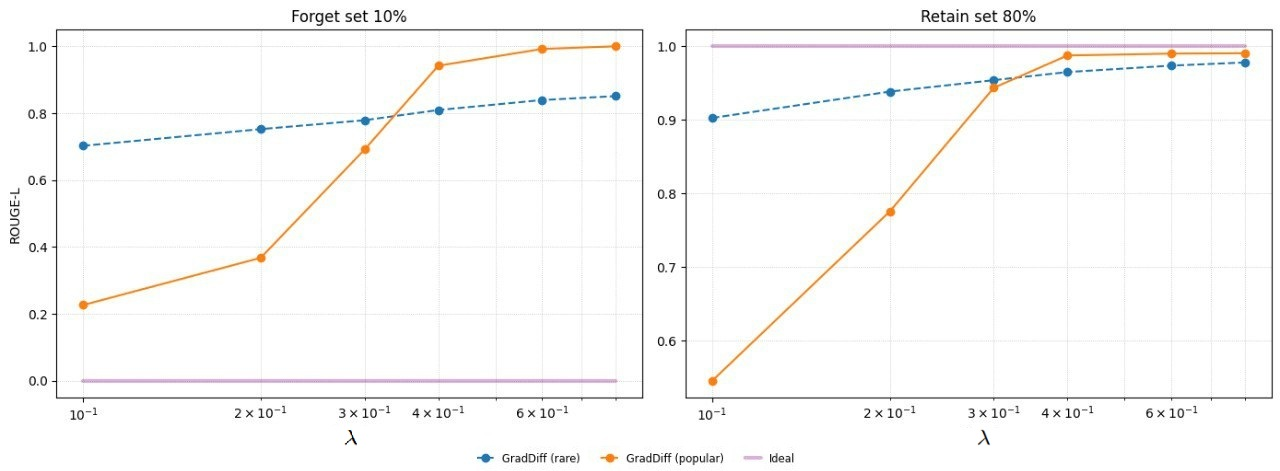
\includegraphics[width=\textwidth]{images/GradDiff_alpha_greedsearch.jpg}
%   \caption{ROUGE-L recall for 10\% rare vs.\ popular facts unlearning with varying alpha (memorization retain set) in Gradient Different unlearning algorithm.}
%   \label{fig:GradDiff_alpha}
% \end{figure*}






% % Heatmap of Tables \ref{tab:split_comparison} and \ref{tab:size_unlearning}: Darker colors indicate \textbf{knowledge retention}, while pale yellow shows \textbf{knowledge forgetting}. Green boxes outline unlearning sets. Black lines separate rare (top) and popular (bottom) validation sets, and fine-tuning from unlearning algorithms. Table \ref{tab:split_comparison} shows \textbf{ineffective learning} at 5\% and \textbf{catastrophic forgetting} at 15\%. Table \ref{tab:size_unlearning} indicates that 1B and 3B models \textbf{poorly acquire and quickly forget information}, irrespective of fact popularity.

% % \begin{figure*}[!ht]
% %   \centering
% %   \includegraphics[width=\textwidth]{images/split_size_heat_map.png}
% %   \caption{Heat map for Table~\ref{tab:split_comparison}: 
% %     Darker colors indicate \textbf{knowledge retention}, pale yellow shows \textbf{knowledge forgetting}.}
% %   \label{fig:split_size_heat_map}
% % \end{figure*}


% % \begin{figure*}[!ht]
% %   \centering
% %   \includegraphics[width=\textwidth]{images/model_size_heat_map.png}
% %   \caption{Heat map for Table~\ref{tab:size_unlearning}: 
% %     Darker colors indicate \textbf{knowledge retention}, pale yellow shows \textbf{knowledge forgetting}.}
% %   \label{fig:model_size_heat_map}
% % \end{figure*}


% % \begin{figure*}[!ht]
% %   \centering
% %   \includegraphics[width=\textwidth]{images/15_unlearning_by_LR.png}
% %   \caption{ROUGE-L recall for 15\% rare vs.\ popular facts unlearning with varying unlearning learning rates.}
% %   \label{fig:15_unlearning_by_LR}
% % \end{figure*}




\clearpage
\appendix
\section{Technical Appendix}
% \section{Supplementary Materials}

% \begin{links}
%     \link{Code}{https://anonymous.4open.science/r/UNLamb_unlearning-B7E4}
%     \link{Benchmark}{https://huggingface.co/datasets/SwetieePawsss/UNLamb}
% \end{links}

% The experimental \textbf{code is hosted anonymously}, and the \textbf{dataset is published} on Hugging Face \textbf{via a purpose-built inactive account} with random username; the repository builds on the OpenUnlearning framework \cite{openunlearning2025}.

Performance on downstream LLM benchmarks (MMLU, HellaSwag) remains largely unaffected following both 5\% and 15\% unlearning (see Table~\ref{tab:llm_unlearn_5_15}). The sole exception is Gradient Ascent at the 15\% level, which exhibits an approximate 30\% reduction in performance—behavior consistent with catastrophic forgetting.


\begin{table}[h!t]
  \centering
  \small
  \setlength{\tabcolsep}{3pt}
  \resizebox{\columnwidth}{!}{%
    \begin{tabular}{|l|c|c|c|c|c|c|c|c|}
      \hline
       & \multicolumn{2}{c|}{\textbf{GradAscent}}
       & \multicolumn{2}{c|}{\textbf{GradDiff}}
       & \multicolumn{2}{c|}{\textbf{NPO}}
       & \multicolumn{2}{c|}{\textbf{RMU}} \\ 
      \hline
       & \textbf{5\%} & \textbf{15\%}
       & \textbf{5\%} & \textbf{15\%}
       & \textbf{5\%} & \textbf{15\%}
       & \textbf{5\%} & \textbf{15\%} \\
      \hline
      \multicolumn{9}{|l|}{\textbf{Rare unlearning}} \\
      \hline
      MMLU $\uparrow$ 
       & 0.548 & 0.382 
       & 0.548 & 0.551 
       & 0.547 & 0.551 
       & 0.533 & 0.519 \\
      \hline
      HellaSwag $\uparrow$ 
       & 0.663 & 0.518 
       & 0.663 & 0.661 
       & 0.663 & 0.658 
       & 0.670 & 0.670 \\
      \hline
      \multicolumn{9}{|l|}{\textbf{Popular unlearning}} \\
      \hline
      MMLU $\uparrow$ 
       & 0.547 & 0.381 
       & 0.548 & 0.538 
       & 0.548 & 0.540 
       & 0.523 & 0.528 \\
      \hline
      HellaSwag $\uparrow$ 
       & 0.663 & 0.603 
       & 0.662 & 0.662 
       & 0.662 & 0.661 
       & 0.667 & 0.668 \\
      \hline
    \end{tabular}%
  }
  \caption{LLMs Performance After 5\% and 15\% Data Unlearning – Rare vs.\ Popular Splits}
  \label{tab:llm_unlearn_5_15}
\end{table}













% \begin{table}[h!t]
%   \centering
%   \small
%   \setlength{\tabcolsep}{3pt}
%   \resizebox{\columnwidth}{!}{%
%     \begin{tabular}{|l|c|c|c|c|c|}
%       \hline
%        & \textbf{FT} & \textbf{GradAscent} & \textbf{GradDiff} & \textbf{NPO} & \textbf{RMU} \\
%       \hline
%       \multicolumn{6}{|l|}{\textbf{Rare unlearning}} \\
%       \hline
%       rare\_forget10 $\downarrow$
%         & 0.458 & 0.246 & 0.321 & 0.321 & 0.324 \\
%       \hline
%       duplicate\_subjects\_rare\_forget10 $\uparrow$
%         & 0.430 & 0.333 & 0.421 & 0.433 & 0.312 \\
%       \hline
%       duplicate\_answers\_rare\_forget10 $\uparrow$
%         & 0.725 & 0.567 & 0.649 & 0.652 & 0.571 \\
%       \hline
%       retain\_intersection80 $\uparrow$
%         & 0.501 & 0.397 & 0.468 & 0.460 & 0.375 \\
%       \hline
%       \multicolumn{6}{|l|}{\textbf{Popular unlearning}} \\
%       \hline
%       popular\_forget10 $\downarrow$
%         & 0.910 & 0.854 & 0.885 & 0.868 & 0.741 \\
%       \hline
%       duplicate\_subjects\_popular\_forget10 $\uparrow$
%         & 0.471 & 0.474 & 0.487 & 0.474 & 0.196 \\
%       \hline
%       duplicate\_answers\_popular\_forget10 $\uparrow$
%         & 0.738 & 0.725 & 0.735 & 0.735 & 0.576 \\
%       \hline
%       retain\_intersection80 $\uparrow$
%         & 0.501 & 0.500 & 0.510 & 0.508 & 0.323 \\
%       \hline
%     \end{tabular}%
%   }
%   \caption{ROUGE-1 recall performance on Gemma-7B for 10\% forget-set size. Top: rare unlearning splits; Bottom: popular unlearning splits.}
%   \label{tab:gemma_unlearn}
% \end{table}




We study how varying the regularization weight \(\lambda\) in Gradient Difference impacts unlearning on the 10\% forget split and observe a pronounced divergence between popular and rare facts (see Figure~\ref{tab:graddiff_lambda_sweep}). Popular facts exhibit a sharp trade-off: small \(\lambda\) values enable forgetting the target set but induce catastrophic forgetting, whereas larger \(\lambda\) values preserve retention at the cost of ineffective unlearning. In contrast, rare facts behave smoothly—there is no abrupt collapse—and tuning \(\lambda\) yields a gradual trade-off between forgetting and retention. These results suggest that unlearning popular facts is substantially more difficult and demands careful, potentially adaptive, selection of \(\lambda\), whereas rare facts are comparatively robust to its setting.


\begin{table}[h!t]
  \centering
  \small
  \setlength{\tabcolsep}{3pt}
  \resizebox{\columnwidth}{!}{%
    \begin{tabular}{|l|c|c|c|c|}
      \hline
       & \multicolumn{2}{c|}{\textbf{Forget 10\% (ROUGE-L $\downarrow$)}} 
       & \multicolumn{2}{c|}{\textbf{Retain 80\% (ROUGE-L $\uparrow$)}} \\ 
      \hline
      $\lambda$ 
       & \textbf{Rare} & \textbf{Popular} 
       & \textbf{Rare} & \textbf{Popular} \\
      \hline
      0.10 & 0.71 & 0.23 & 0.90 & 0.54 \\
      0.20 & 0.74 & 0.38 & 0.92 & 0.78 \\
      0.30 & 0.77 & 0.68 & 0.94 & 0.94 \\
      0.40 & 0.80 & 0.92 & 0.96 & 0.99 \\
      0.60 & 0.82 & 0.98 & 0.97 & 1.00 \\
      \hline
    \end{tabular}%
  }
  \caption{GradDiff sensitivity to the regularization weight $\lambda$ on the 10\% forget and 80\% retain splits.}
  \label{tab:graddiff_lambda_sweep}
\end{table}


%%%%%%%% fig:GradDiff_alpha
% \begin{figure*}[!ht]
%   \centering
%   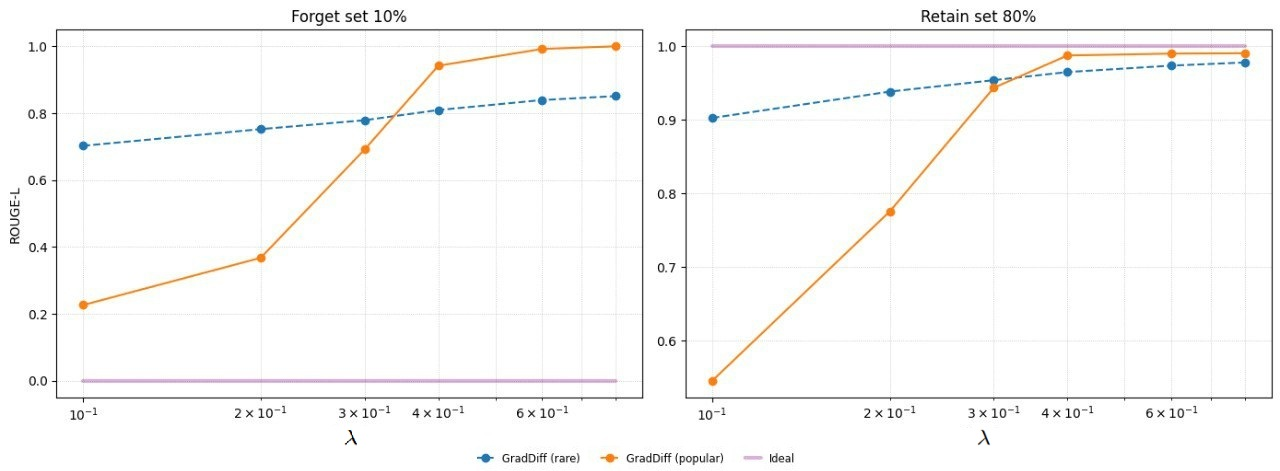
\includegraphics[width=\textwidth]{images/GradDiff_alpha_greedsearch.jpg}
%   \caption{ROUGE-L recall for unlearning 10\% rare vs.\ popular facts with varying \(\lambda\) (retain-set regularization weight) in the Gradient Difference algorithm.}
%   \label{fig:GradDiff_alpha}
% \end{figure*}






% Heatmap of Tables \ref{tab:split_comparison} and \ref{tab:size_unlearning}: Darker colors indicate \textbf{knowledge retention}, while pale yellow shows \textbf{knowledge forgetting}. Green boxes outline unlearning sets. Black lines separate rare (top) and popular (bottom) validation sets, and fine-tuning from unlearning algorithms. Table \ref{tab:split_comparison} shows \textbf{ineffective learning} at 5\% and \textbf{catastrophic forgetting} at 15\%. Table \ref{tab:size_unlearning} indicates that 1B and 3B models \textbf{poorly acquire and quickly forget information}, irrespective of fact popularity.

% \begin{figure*}[!ht]
%   \centering
%   \includegraphics[width=\textwidth]{images/split_size_heat_map.png}
%   \caption{Heat map for Table~\ref{tab:split_comparison}: 
%     Darker colors indicate \textbf{knowledge retention}, pale yellow shows \textbf{knowledge forgetting}.}
%   \label{fig:split_size_heat_map}
% \end{figure*}


% \begin{figure*}[!ht]
%   \centering
%   \includegraphics[width=\textwidth]{images/model_size_heat_map.png}
%   \caption{Heat map for Table~\ref{tab:size_unlearning}: 
%     Darker colors indicate \textbf{knowledge retention}, pale yellow shows \textbf{knowledge forgetting}.}
%   \label{fig:model_size_heat_map}
% \end{figure*}


% \begin{figure*}[!ht]
%   \centering
%   \includegraphics[width=\textwidth]{images/15_unlearning_by_LR.png}
%   \caption{ROUGE-L recall for 15\% rare vs.\ popular facts unlearning with varying unlearning learning rates.}
%   \label{fig:15_unlearning_by_LR}
% \end{figure*}